\chapter{Beginner's Algorithm}\label{chap:beginnerImplement}
\myTop{In this chapter the process of implementing beginner's algorithm, which is described in section \ref{sec:beginner}, will be presented.
This implementation will not be as effective as beginner's algorithm is capable of since it is a proof of concept.
How efficient it is will be presented in form of statistics about the number of twists it needs to solve the Rubik's Cube.}
This chapter is divided into the different steps used in the beginner's algorithm.
Each step is using different algorithms which all are generally structured in the same way. 

For the sake of simplicity the first layer (down face) in our implementation will always be the same face. We have chosen that face to be the yellow face, the green is the front face, and the red is the right face. This will make the implementation process easier, but the solution will require more twists since it is unlikely that the yellow face is the optimal choice as the first layer face for every solve.

The implementation uses several algorithms which all are named algorithm XnN, where Xn is the step that the algorithm is used in and N is used to distinguish the algorithms from each other, which are used in the same step.

Most of them contains a \textbf{switch-case} statement which is dependent on some input specified for each algorithm. In all cases this is based on the point of view. Normally a human will simply rotate the whole \cube{} and perform the same algorithm, but we found it easier simply to define the algorithms from the different locations.

\section{The Steps}
In the following the implementation of the steps of the beginner's algorithm will be described.
The steps are based on the steps described in section \ref{sec:beginner}. 
\subsection{Step 1 -- Getting the Cross}
\section{Step 1 -- the First layer Cross}
The first question our program needs to ask is whether the edge pieces already are positioned correctly. If that is the case and the edge piece is also oriented correctly, the program proceeds to the next edge piece. If not an algorithm is performed, which changes the edge piece's orientation without ruining other possibly correctly positioned edge pieces(This algorithm will be known as "`algorithm 1"'). When the edge piece is in the the correct position and has the correct orientation, the program moves on to another edge piece. 

If the edge \cpiece{} in question is not in it's correct position, the program needs to know where the edge is positioned. 
The way this is done is by first checking if the edge \cpiece{} is positioned in the first layer. 
If this is the case the edge \cpiece{} in question is moved to the opposite layer. 
If the edge \cpiece{} is not in the first layer it can either be in the opposite layer or in the second layer.
Is the edge piece positioned in the second layer an algorithm is performed which moves the edge piece to the white layer, which is the opposite of the layer in which we make the cross.

Now that the edge piece is in white layer it needs to be moved to the position directly above where it is correctly positioned. 
The program does this by twisting the up face once (known as an U move) and checks if the edge piece is above it's correct position.
The edge piece is now positioned in two faces -- the white face and the face which has the same color as the edge piece's second \facelet{} i.e. the face that is not yellow.
In order to position the edge piece correctly that face is twisted twice.
The edge piece is now in it's correct position, and if it is oriented correctly the program moves on to another edge piece.
If the edge piece is oriented incorrectly algorithm 1 is performed. If more edge pieces needs to be positioned or oriented correctly the program will continue with the same method until the cross is finished in which case the program moves on to the next step.

%INSERT FLOWCHART
\subsection{Step 2 -- Completing the First Layer}
\section{Step 2 -- completing the first layer}
This step fits the first layer corners into place. The method used for this is very similar to the methods of step 1. 
As with step one the algorithm starts with a specific cube and then try to fit this into place. 
The step is generally described in subsection \ref{sub:step2}.

First it checks whether the cube is already in the right place, if so and it is not correctly orientated an algorithm denoted \textit{algorithm 3} will ``rotate'' this \cpiece{} in its spot until the orientation is correct. 

If the cube is somewhere else in the down layer then an algorithm will move it up to the top layer. 
By now we know that the corner \cpiece{} is either placed correct or is in the white layer. 
The up face will be twisted until the \cpiece{} is placed directly above its correct place. 
Then the same algorithm used to move the cube up will now move it down. 
\textit{Algorithm 3} is then run until the cube is oriented correctly.

\subsection{Step 3 -- Solving the Second Layer}
\section{Step 3 -- solving the second layer}
In this step the second layer will be solved. 
This means that the edges in the second or middle layer will get placed and orientated correctly. 
In subsection \ref{sub:step3} this is step is generally described. 

The program solve this layer by going through the 4 \cubicle{}s of the second layer and finding and placing the \cpiece{} in its \cubicle{}

If the \cpiece is oriented incorrectly in the correct \cubicle{} the program will use an algorithm to move the edge \cpiece{} to the top layer and move it back to the same position -- but now the orientation will be correct. 

If the edge \cpiece{} is not in it's correctly position the program needs to know where the correct edge piece is positioned. First the program checks for it in the top layer. 
If it is in the top layer up moves are applied to the \rubik{} until the edge piece is positioned in such a way that an algorithm can be applied to move it to it's correct position with the correct orientation. 
If the \cpiece{} is in the second layer but in a wrong \cubicle{} the same algorithm used to put it into place will get it out of place. 



\subsection{Step 4a --  Getting the Last Layer Cross}
\section{Step 4 --  getting the last layer cross}
In the previous steps the algorithms has solved one \cpiece{} at a time. 
This is not an option for this step. 
Here several \cpiece{}s will be placed at a time. 

This step will make the orientation of the top face cross correct. 
Placing the \cpiece{}s correctly will first be done in the next. 
This is done by checking each case of possible orientation for the edge \cpiece{}s in the top layer. 
There are 3 primary positions where different actions should be taken. See figure \ref{fig:cross}. 
\begin{enumerate}
\item L - shape
\item None is up.
\item A row
\end{enumerate}
It is \textit{algorithm 8} that needs to be performed no matter the case. In case one the algorithm is applied twice, case two the algorithm is applied three times, case 3 the algorithm is applied 1 time. 

\ref{fig:cross}



\subsection{Step 4b -- Completing the Last Layer Cross}
\section{Step 5 -- Completing the Last Layer Cross}
In the theoretical description of the beginner's algorithm step five is the implementation's step five, six and seven. 
In this step the edges of the last layer cross will be positioned correctly. Their orientation will not be changed, since they are already oriented correctly. See subsection \ref{sub:step5}.

The four \cpiece{}s in the white layer cross can only be in the four \cubicle{}. This leaves us with essentially two cases. Either all \cpiece{}s are placed correctly or two are placed correctly. This requires twisting the up face until one of these cases will appear.

The program only needs to respond to the case where two \cpiece{}s are placed correctly. 
If the the two correctly positioned edges are positioned directly across each other \textit{algorithm 9} is performed.
The correctly positioned edge \cpiece{}s are now on two faces next to each other. This is either reached by \textit{algorithm 9} or they were already positioned this way.
The program checks which two edge \cpiece{}s are positioned correctly and performs \textit{algorithm 9} accordingly. 
The edges are now positioned and oriented correctly and the program moves on to the next step.
\subsection{Step 5a -- Positioning the Last Layer Corners}
<<<<<<< .mine
\section{Step 6 -- placing the last layer corners}
In this step the corners in the last layer will be positioned correctly. 
The basic theory of the cases in this step is similar to the ones in step five.

The initial action performed is a check of the number of correctly positioned corner \cpiece{}s. 
If all four corner \cpiece{}s are positioned correctly the program moves on to the next step.
If none of the corners are positioned correctly \textit{algorithm 10} is performed. This will position one of the corner \cpiece{}s correctly.
When one corner is positioned correctly, then the program will perform \textit{algorithm 10} based on what corner is positioned correctly.
Now the program will perform a check again to see if all the corners are positioned correctly. If all the four corners are not positioned correctly \textit{algorithm 10} will be performed again.
When that is done all the four corner \cpiece{}s are positioned correctly and we can move on to the last step.
=======
\section{Step 6 -- placing the last layer corners}
In this step the corners in the last layer will be positioned correctly. 
The basic theory of the cases in this step is similar to the ones in step five.

The initial action performed is a check of the number of correctly positioned corner \cpiece{}s. 
If all four corner \cpiece{}s are positioned correctly the program moves on to the next step.
If none of the corners are positioned correctly \textit{algorithm 10} is performed. This will position one of the corner \cpiece{}s correctly.
When one corner is positioned correctly, then the program will perform \textit{algorithm 10} based on what corner is positioned correctly.
Now the program will perform a check again to see if all the corners are positioned correctly. If all the four corners are not positioned correctly \textit{algorithm 10} will be performed again.
When that is done all the four corner \cpiece{}s are positioned correctly and we can move on to the last step.
>>>>>>> .r884

\subsection{Step 5b -- Completing the Last Layer}
\section{Step -- Solving last layer orientation}
This is the last step and when the algorithm gets to this step everything is placed correctly, the corners of the last layer only needs to be orientated correctly.

The algorithm takes one corner at a time and checks this orientation. This is alway the up right front corner. If it orientated wrongly algorithm 10 is applied, this algorithm rotates a corner without ruining the rest of the \cube{}. When the corner is correctly orientated the U face is \twist{}ed so a new corner is placed in this position and the same procedure is applied. After four U turns and appliance of algorithm 10 the cube is finally solved. 



\begin{comment}
In the last layer the corners in the last layer were poisitend correctly but not oreiented. In this step will the coreners be oreinted correctly and as result it will lead to that the \rubiks{} will be solved.

This step is very simple because it there is only four corners to control and either the corner is oriented correctly or is isn't.  

The program vil first control that the front-right-up corner is oriented correctly if not the will use the an algorithm twice and after the program vil control the corner again if the corner is not oriented correctly his time the use teh algorithme and will continue with this until the corner is oriented correctly. 
Then the corner is orented correctly the program will make at up move ("U") and will control the new corner and the program will do this with every corner in the last layer until they are oriented corectly.  

\end{comment}
%husk flow diagram 

\section{Twist Reduction}
As mentioned before our implementation of the beginner's algorithm is not as efficient as it can be. We can however take some steps towards improving its efficiency. One of these steps is removing unnecessary moves and replacing a move sequence with a shorter move sequence, which gives the same result.

An unnecessary move sequence can be performing a twist and just after that twist perform its inverse move. e.g. performing \m{U U'} or \m{U' U}.
According to the theory of groups in section \ref{sec:groupDefinition} two moves, which are each other's inverse give the same result as not performing the two moves.

It was necessary to be able to shorten the twists generally, so any move sequence can not be replaced with a shorter one in our program.
An example of replacing a move sequence with a shorter one generally is replacing three of the same type of move with a single inverse move of that type. e.g. \m{U U U} also noted as \m{U2 U} or \m{U U2} can be replaced with a single inverse move \m{U'}. This is also described in the group theory section \ref{sec:groupDefinition}.

\section{Statistics for Beginner's Algorithm}
\label{sec:beginnersStat}
In order to get the average length of a solution of beginner's algorithm we must determine how many moves of scrambling must be applied in order to find the worst case scenario. 
By computing the average for different amount of scrambles the graph quickly becomes steady at around 40 scrambles (10.000 cubes is tested) (see figure \ref{fig:beginnersScramble}). To be sure that we get a good result we go by 50 scrambles.
\begin{figure}[htbp]
	\centering
		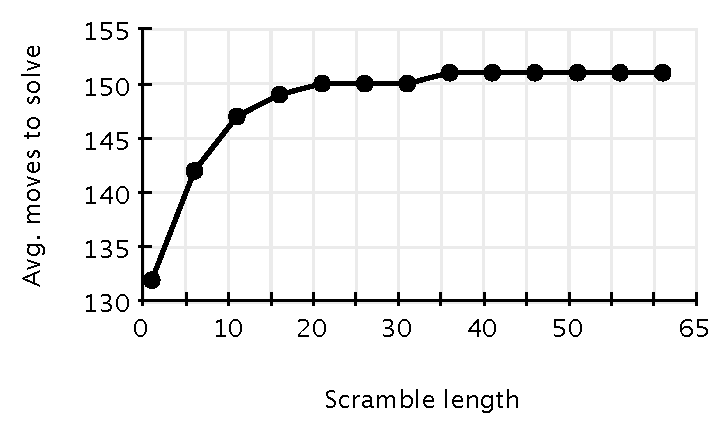
\includegraphics{input/pics/beginnersScramble.pdf}
	\caption{\myCaption{The graph shows the amount of moves needed to solve a cube with x scrambles. The lines are for showing only and do not represent the average between the dots.}}
	\label{fig:beginnersScramble}
\end{figure}

Now that the number of scrambles is determined the average number of \twist{}s can be found.
By scrambling 10 million \cube{}s and solve them with the beginner's algorithm we get an average of \textbf{151 moves}.
A test using only 1 million \rubik{}s is run three times in order to insure that the test is reliable.
The raw data from both tests is found in appendix \ref{chap:beginnerResults}.
%Which is the average of beginner's algorithm.
The maximum value found is 241 moves and minimum is 56 moves. 



The data was gathered on a computer operated by Windows 7 64 bits running on a 2.5 GHz AMD Quad Core processor (905e) with 4 GB DDR-3 RAM.

A peculiar note is that with one twist, the algorithm needs an average of 132 moves with a maximum of 155 and a minimum 94 moves to solve it again.
This illustrates the twist-wise inefficiency of this algorithm very well.


\myTail{In this chapter the implementation of beginner's algorithm is described.
Statistics about our implementation is gathered in order to compare this algorithm to our implementation of Kociemba's optimal solver.}